\section{Lezione 12}%
\label{sub:Lezione 12}
\subsection{Simulazione del processo di Wiener in una doppia buca.}%
\label{sub:Simulazione dei camminatori.}
Riprendiamo l'ultimo argomento della lezione \ref{sub:Parte 2}, ovvero il calcolo del tempo di primo passaggio con un metodo più potente. \\
Prendiamo un sistema di camminatori che seguono la seguente SDE:
\begin{equation}
\begin{aligned}
    dx = & f(x) dt + \sqrt{\epsilon} dW = \\
    = & \left(x-x^3\right)dt + \sqrt{\epsilon} dW
.\end{aligned}
\label{eq:12_beg}
\end{equation}
In cui $f(x)$ è la forza che sente il camminatore in un potenziale a doppia buca della forma:
\begin{figure}[H]
    \centering
    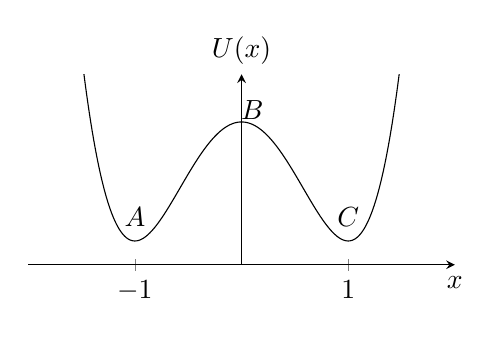
\begin{tikzpicture}
	\begin{axis}[
	    width=7cm,
	    height=4cm,
	    xmin= -2, xmax= 2,
	    ymin= 0, ymax = 0.4,
	    axis lines = middle,
	    x label style={at={(axis description cs:1,-0.01)},anchor=north},
	    y label style={at={(axis description cs:0.5,1)},anchor=south},
	    xlabel={$x$},
	    ylabel={$U(x)$ },
	    xtick={0, 1, -1},
	    xticklabels={$0$, $1$, $-1$},
	    ytick={0},
	    yticklabel={$0$},
	    ]
	    \addplot[domain=-3:3, samples=500]{-x^2/2*(1-x^2/2) + 0.3};
	    \node (C) [mark=dot] at (axis cs: 1, 0.1) {$C$};
	    \node (B) [mark=dot] at (axis cs: 0.1, 0.325) {$B$};
	    \node (A) [mark=dot] at (axis cs: -1, 0.1) {$A$};
	\end{axis}
    \end{tikzpicture}
    \caption{\scriptsize Potenziale in cui vivono i camminatori (l'integrale di $f$ con il segno invertito).}
    \label{fig:lore}
\end{figure}

\noindent
Ipotizziamo di inserire tutti i camminatori nel punto $A$, il sistema grazie al processo di Wiener $dW$ inizia a muoversi e può capitare che un camminatore riesca a raggiungere il punto $B$ cadendo poi nella buca con minimo in $C$. \\
Quello che vogliamo capire è se tutti i processi di Wiener possono permettere questo tipo di moto oppure se serve una configurazione particolare di $dW_n$ per raggiungere la buca $C$. Per capirlo operativamente si eseguono i seguenti passaggi:
\begin{itemize}
    \item Si simula il sistema ipotizzando $\sqrt{\epsilon} \ll f(x) \ \forall x$.
    \item ad evoluzione finita si considerano solo le traiettorie $x^{(j)}$ che hanno raggiunto $C$ al tempo $t^{(j)}$.
    \item Si trasla l'origine temporale di ogni traiettoria $x^{(j)}$ nell'istante in cui tale traiettoria ha raggiunto $C$.
    \item Si graficano tutte le traiettorie in un unico plot.
\end{itemize}
Effettuando una simulazione multipla seguendo questo procedimento si ottiene:
\begin{figure}[H]
    \centering
    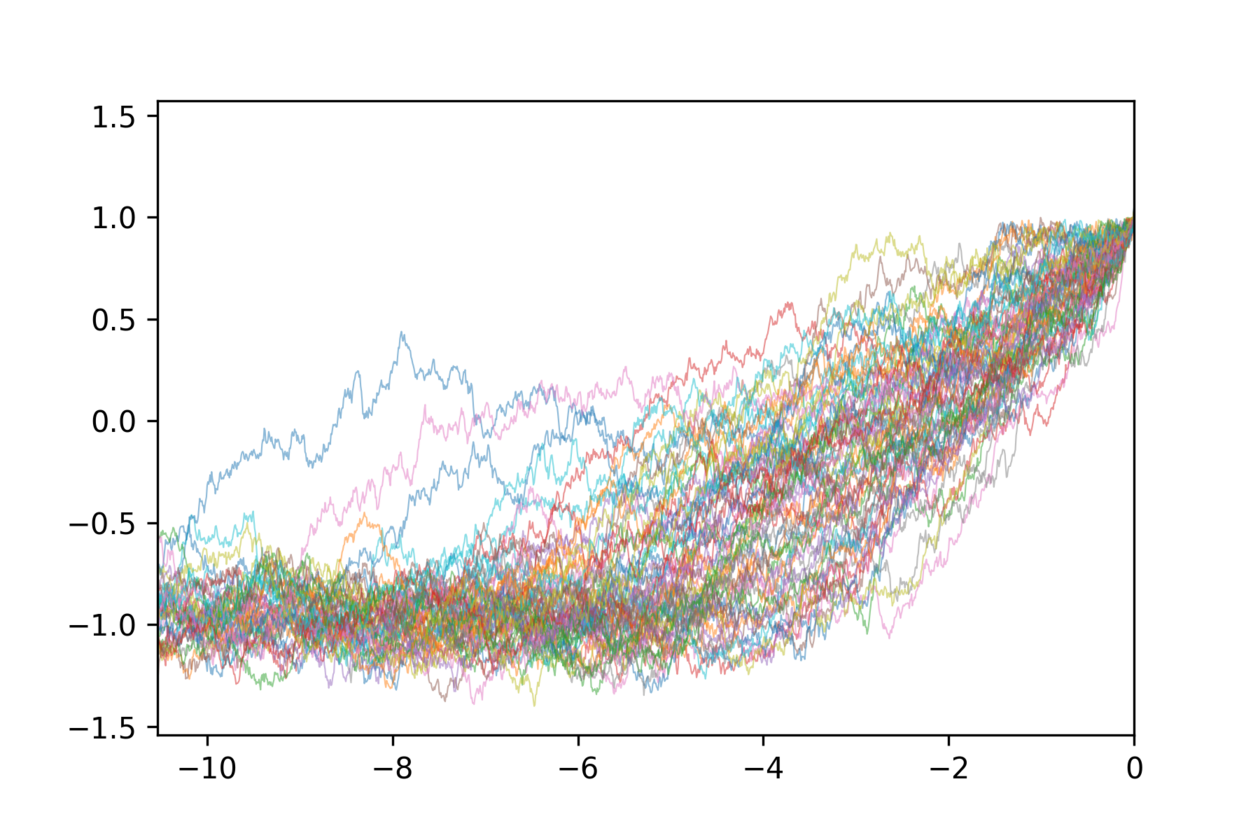
\includegraphics[width=0.5\textwidth]{figures/lez_12_walker_t_path.png}
    \caption{\scriptsize 70 camminatori che raggiungono il punto C (\href{https://github.com/dodogabrie/Sistemi-Complessi/blob/master/python-project/lezione12/MFPT_simulation_py.ipynb}{Link al codice in python}).}
    \label{fig:figures-lez_12_walker_t_path-png}
\end{figure}
\noindent 
Si nota come tutte le traiettorie sembrino seguire un percorso specifico, incanalandosi in una specie di tubo di flusso per arrivare in $x=1$. \\
Questa cosa appare evidente se andiamo a vedere la densità dei punti in cui nei quali è passato il camminatore:
\begin{figure}[H]
    \centering
    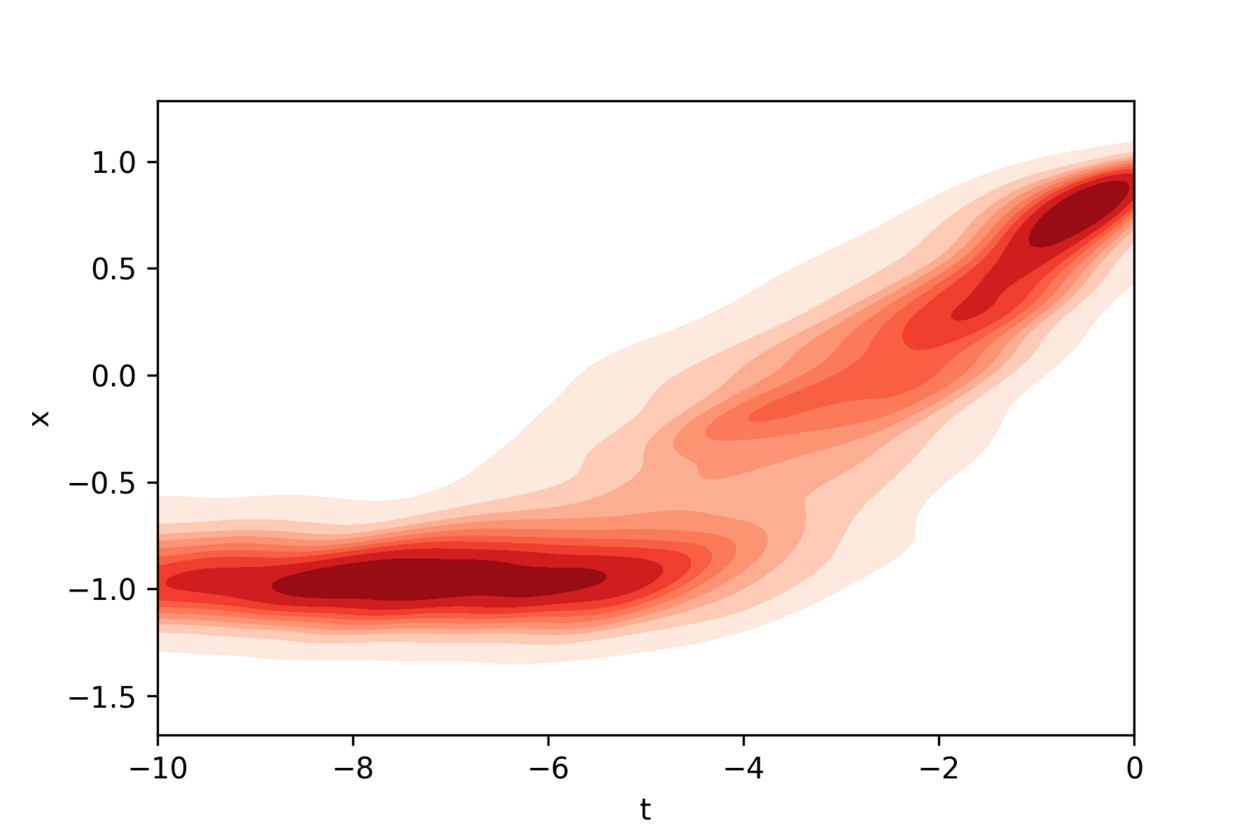
\includegraphics[width=0.5\textwidth]{figures/lez_12_walker_t.png}
    \caption{\scriptsize Densità dei camminatori che riescono a fare il salto nel tempo, si nota che si addensano attorno ad un tubo di flusso (\href{https://github.com/dodogabrie/Sistemi-Complessi/blob/master/python-project/lezione12/MFPT_simulation_py.ipynb}{Link al codice in python})}
    \label{fig:figures-lez_12_walker_t-png-}
\end{figure}
\noindent 
Una cosa molto interessante da notare è la scala temporale, se mediamente un camminatore impiega un tempo di $100$ digit per scappare dalla buca $A$ restringendoci ai soli camminatori che riescono nell'impresa questo tempo risulta essere inferiore a $8$ digit. \\
Questo significa che la sequenza di $dW_n$ che permette il passaggio è molto improbabile, infatti deve essere tale da spingere il camminatore oltre una barriera!\\
Si possono prendere tutte le sequenze di $dW$ che hanno permesso ai $70$ camminatori di attraversare la barriera e valutarne la densità in $x$. Il seguente grafico mostra un istogramma bidimensionale ('countour plot') del rumore in funzione di $x$:
\begin{figure}[H]
    \centering
    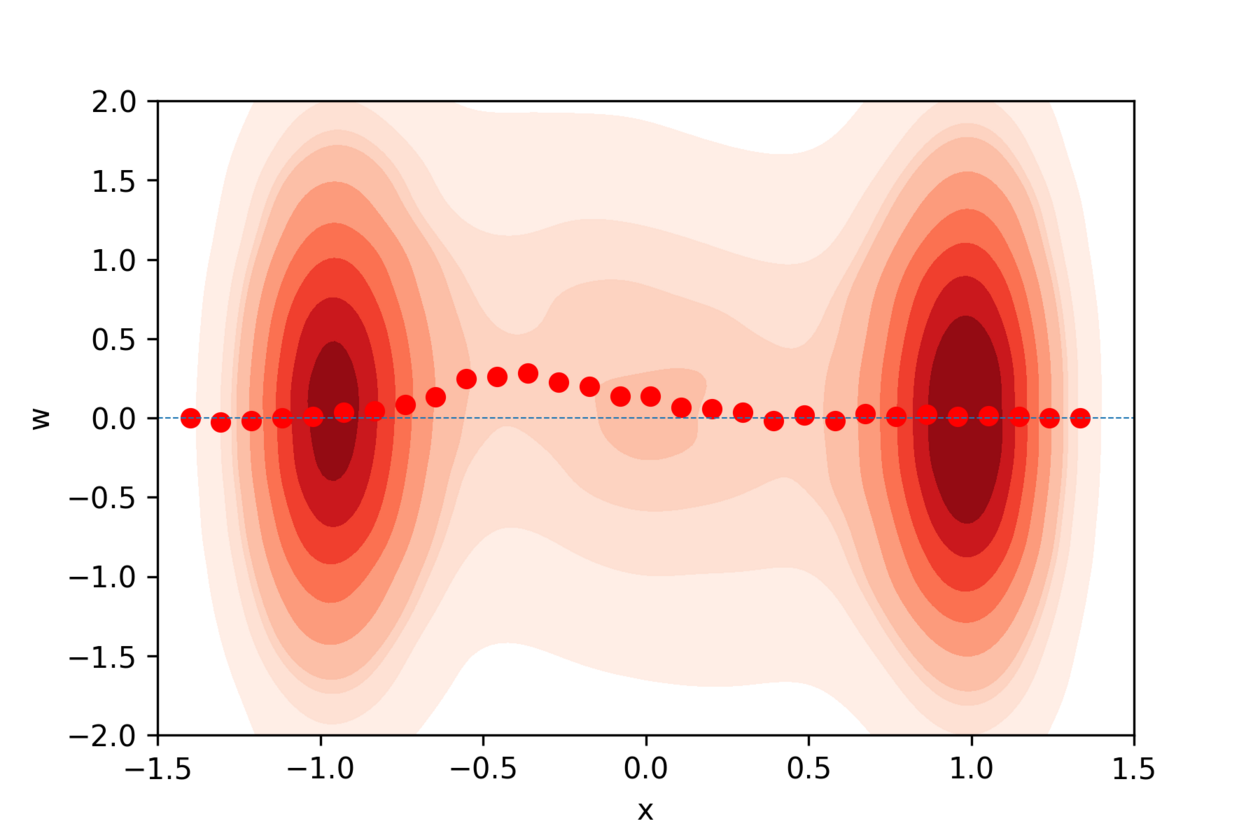
\includegraphics[width=0.5\textwidth]{figures/lez_12_dist.png}
    \caption{\scriptsize Distribuzione del processo stocastico per i camminatori che riescono a fare il salto, notiamo che la media del processo (curva arancione) deve essere diversa da zero (\href{https://github.com/dodogabrie/Sistemi-Complessi/blob/master/python-project/lezione12/MFPT_simulation_py.ipynb}{Link al codice in python}).}
    \label{fig:figures-lez_12_dist-png}
\end{figure}
\noindent
Possiamo notare il fatto che per ottenere una sequenza giusta il rumore debba essere diverso da zero (e positivo) lungo la salita del potenziale. \\
Superata la barriera allora il rumore può gradualmente rilassare: la fatica ormai è fatta. 

\subsection{Hamiltoniana per il MFPT}%
\label{sub:Hamiltoniana per il MFPT}
Riprendiamo l'equazione per il processo in forma discretizzata:
\[
    x_{n+1} = x_n + f(x_n) \Delta t + \sigma \Delta\omega_n = F(x_n) + \xi_n
.\] 
\[
    \left<\xi_n\xi_m\right> = \epsilon\Delta_{nm}
.\] 
Consideriamo sempre l'intervallo $(a,b)$ come sopra. Abbiamo visto che la probabilità di andare da $a$ a $b$ 
\[
    P\left(x_b,t|x_a,0\right)
.\] 
è legata alla probabilità di una "corretta" fluttuazione di $\xi$. \\
Supponiamo di discretizzare il tempo con un passo $\Delta t$:
\[
    t_{i+1} = t_i + \Delta t 	\quad \forall i
.\] 
La probabilità di arrivare in $b$ può essere scritta come una catena di propagatori:
\[\begin{aligned}
    P\left(x_b,t|x_a,t_0\right)=&P\left(x_1,t_1|x_a,t_0\right)\cdot P\left(x_2,t_2|x_1,t_1\right)\cdot \ldots \\
				&\ldots \cdot P\left(x_b,t_b|x_{n-1},t_{n-1}\right)
.\end{aligned}\]
Dove si sfrutta in questo passaggio il fatto che il sistema è markoviano (quindi è lecito scrivere la probabilità composta in questo modo).\\
Notiamo che la probabilità di fare il salto dalla posizione $x_{i}$ a quella $x_{i+1}$ deve essere legato alla probabilità di ottenere il "giusto" $\xi_i$  del processo di Wiener:
\[
    P\left(x_{i+1}, t_{i+1}|x_i,t_i\right) \sim P(\xi_i) 
.\] 
\[
    \text{Con } \xi_i: \quad x_{i+1} = F(x_i) + \xi_i
.\] 
Sia $\gamma$ una fluttuazione ottimale che permette il passaggio da $a$ a $b$.
\[
	\gamma \to \left[\zeta_1, \ldots, \zeta_n\right]
.\] 
La probabilità che tale fluttuazione avvenga avrà la forma (vedi ad esempio la soluzione stazionaria della Lezione \ref{eq:5_staz}):
\[
    P(\gamma) \sim \exp\left(-\frac{S\left[x_1,\ldots,x_n\right]}{\epsilon}\right)
.\] 
\[
    S = \frac{1}{2}\sum_{}^{} \zeta^2_i
.\] 
Quindi il tempo di primo passaggio può essere ricavato dal fatto che
\footnote{La dimostrazione che questa probabilità ed il MFPT sono legati è nel PDF del professore (pathintegral).}
:
\[
    P\left(x_n,t_n = T|x_0,t_0\right) \sim k \exp\left(-\frac{S_{\text{min}}}{\epsilon}\right)
.\] 
Quello che cerchiamo è il minimo dell'azione $S$: $\overline{S}$, ovvero la sequenza $\gamma$ che massimizza la probabilità di fare il salto $a\to b$.\\
Per risolvere il problema di minimo possiamo utilizzare un set di moltiplicatori di Lagrange $\lambda_i$.
\[
    \overline{S} = \frac{1}{2}\sum_{i}^{} \zeta^2_i + \lambda_i \left[x_{i+1}-F(x_i)- \zeta_i\right]
.\] 
Risolvendo il problema dei moltiplicatori si ottiene:
\[\begin{aligned}
    &1. \quad x_{n+1} = F(x_n) + \lambda_n\\
    &2. \quad \lambda_{n+1}=\left[\left.\frac{\partial F}{\partial x_i} \right|_{i = n+1}\right]^{-1}\lambda_n
.\end{aligned}\]
Passiamo a tempi continui, chiamiamo $\Delta t = h$, dalla prima equazione si ottiene che
\footnote{Non mi torna l'$h$, mi pare sparita\ldots}
:
\[
    x_{n+1} = x_n + h f(x_n) + \lambda_n \implies  \dot{x} = f + \lambda
.\] 
La seconda equazione può essere manipolata considerando la definizione di $F$:
\[
    F(x_n) = x_n+hf(x_n) \quad \implies  \quad  \frac{\partial F}{\partial x} = 1+hf'
.\] 
Sostituendo questa nella (2.) e sommando e sottraendo $\lambda_n$ si arriva a:
\[
    \dot{\lambda} =  - f'\lambda
.\] 
Ci siamo ricondotti a due equazioni da integrare con le opportune condizioni al contorno:
\begin{redbox}{Equazioni di Hamilton per il sistema}
\[
    \begin{cases}
	\dot{x} = f(x) + \lambda\\
	\dot{\lambda } = - f'(x) \lambda
    \end{cases}
.\]     
\end{redbox}
\noindent
l'Hamiltoniana che corrisponde a queste equazioni è della forma:
\[
    \lambda  \to p \quad \implies  \quad H = \frac{p^2}{2} + pf
.\] 
Infatti vale che:
\[
    \begin{cases}
	\dot{x} = \left[x,H\right]\\
	\dot{p} = \left[p,H\right]
    \end{cases}
.\] 
Le condizioni al contorno che possiamo usare per risolvere sono 
\[
    x(t=0) = a; \quad x(t = t_n) = b
.\] 
Il problema può essere risolto con il calcolo della azione, sappiamo che l'azione di un sistema è legata alla lagrangiana dalla seguente:
\[
    \dot{S} = \mathcal{L} = \frac{\partial H}{\partial P} P - H
.\] 
Quindi operativamente basta integrare la lagrangiana per ottenere la $S$, minimizzarla per avere la $P$, visto che $P$ è proporzionale al tempo di primo passaggio $T$. 
\subsubsection{Applicazione del metodo ad un potenziale $U(x)$}%
\label{subsub:Applicazione del metodo ad un potenziale $U(x)$}
Prendiamo l'equazione per l'incremento di $x$:
\[
    dx = - U' dt + \sqrt{\epsilon} d\omega
.\] 
In cui si ha che, come già accennato $-U' = f$:
\[
    H = \frac{p^2}{2}-pU'
.\] 
Risolviamo le equazioni di Hamilton:
\[
    \begin{cases}
	\dot{x} = -U' + p\\
	\dot{p} = U''p
    \end{cases}
.\] 
Possiamo derivare la prima e sostituire $\dot{p}$ dalla seconda:
\[\begin{aligned}
    \ddot{x} &= -U'' \dot{x} + \dot{p} =\\
	      & = - U'' \dot{x} + U'' p = \\
	      & = U''\left(- \dot{x} + p\right) = U'U''
.\end{aligned}\]
Quindi ne emerge che $U'U''$ ha la struttura di una "forza"
\footnote{Per unità di massa eventualmente\ldots}, 
vediamo qual'è la forma grafica di tutte le quantità in gioco.
\begin{figure}[H]
    \centering
    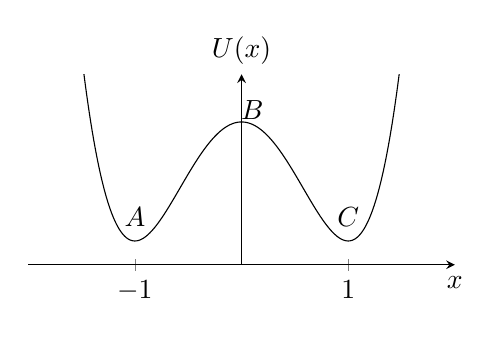
\begin{tikzpicture}
	\begin{axis}[
	    width=7cm,
	    height=4cm,
	    xmin= -2, xmax= 2,
	    ymin= 0, ymax = 0.4,
	    axis lines = middle,
	    x label style={at={(axis description cs:1,-0.01)},anchor=north},
	    y label style={at={(axis description cs:0.5,1)},anchor=south},
	    xlabel={$x$},
	    ylabel={$U(x)$ },
	    xtick={0, 1, -1},
	    xticklabels={$0$, $1$, $-1$},
	    ytick={0},
	    yticklabel={$0$},
	    ]
	    \addplot[domain=-3:3, samples=500]{-x^2/2*(1-x^2/2) + 0.3};
	    \node (C) [mark=dot] at (axis cs: 1, 0.1) {$C$};
	    \node (B) [mark=dot] at (axis cs: 0.1, 0.325) {$B$};
	    \node (A) [mark=dot] at (axis cs: -1, 0.1) {$A$};
	\end{axis}
    \end{tikzpicture}
    \begin{tikzpicture}
	\begin{axis}[
	    width=7cm,
	    height=4cm,
	    xmin= -2, xmax= 2,
	    ymin= -0.4, ymax = 0.4,
	    axis lines = middle,
	    x label style={at={(axis description cs:1,0.49)},anchor=north},
	    y label style={at={(axis description cs:0.5,1)},anchor=south},
	    xlabel={$x$},
	    ylabel={$U'(x)$ },
	    xtick={0, 1, -1},
	    xticklabels={$0$, $1$, $-1$},
	    ytick={0},
	    yticklabel={$0$},
	    ]
	    \addplot[domain=-3:3, samples=500]{-x+x^3};
	\end{axis}
    \end{tikzpicture}
    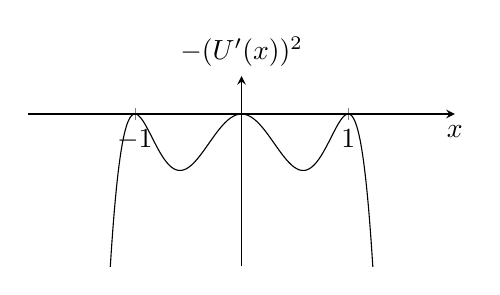
\begin{tikzpicture}
	\begin{axis}[
	    width=7cm,
	    height=4cm,
	    xmin= -2, xmax= 2,
	    ymin= -0.4, ymax = 0.1,
	    axis lines = middle,
	    x label style={at={(axis description cs:1,0.79)},anchor=north},
	    y label style={at={(axis description cs:0.5,1)},anchor=south},
	    xlabel={$x$},
	    ylabel={$-(U'(x))^2$ },
	    xtick={0, 1, -1},
	    xticklabels={$0$, $1$, $-1$},
	    ytick={0},
	    yticklabel={$0$},
	    ]
	    \addplot[domain=-2:2, samples=500]{-1*(-x+x^3)^2};
	\end{axis}
    \end{tikzpicture}
    \caption{\scriptsize Potenziale in cui vivono i camminatori e la sua derivata strettamente legata alla forza sul camminatore.}
    \label{fig:12_pot_der}
\end{figure}

\noindent
Il potenziale efficace che mi genera la forza $U'U''$ è 
\[
    U_{\text{eff}} = -\frac{1}{2}\left(U'(x)\right)^2
.\] 
Questo perché effettuando tale derivata si riottiene l'equazione sopra ai grafici, si ha quindi:
\[
    \ddot{x} = \frac{\text{d} }{\text{d} x} \left(-\frac{1}{2}(U'(x) ) ^2\right)
.\] 
Quindi se integriamo questa equazione in $x$ si scopre che il moto avviene ad una energia costante $E$, di fatto si trova la conservazione della energia meccanica:
\[
    \frac{1}{2} \dot{x}^2 - \frac{1}{2} U'^2 = E
.\] 
Notiamo che il grafico che conta ai fini del moto (della velocità del camminatore) è il terzo in Figura \ref{fig:12_pot_der}.\\
Poniamoci nel caso di energia nulla, si ottiene che
\begin{equation}
    \dot{x} = \pm U'
    \label{eq:12_moto}
\end{equation}
Fisicamente nel sistema	si ha che nel tratto di salita sul potenziale l'equazione del moto è 
\[
    \dot{x} =  + U'
.\] 
Mentre nel tratto di successiva discesa vale l'equazione con il meno. In conclusione si ha per l'esempio discusso in questa lezione:
\[
    \begin{cases}
	\dot{x} = + U' & x<0\\
	\dot{x} = -U' & x\ge 0
    \end{cases}
\] 
Adesso possiamo confrontare questa equazione con quella di partenza di questa lezione (è la \ref{eq:12_beg} riscritta):
\[
    \dot{x} = -U' + \xi
.\] 
Quindi notiamo che nella parte di discesa il moto stocastico $\xi$ è irrilevante, infatti abbiamo l'equazione di partenza con $\xi=0$. Nella parte di salita invece il moto stocastico è tale da invertire di segno all'equazione per $ \dot{x}$.\\
Proprio per questo motivo le sequenze che permettono il passaggio sopra la barriera sono difficili da generare.
Possiamo allora confrontare questa soluzione con le simulazioni mostrate sopra, generando la traiettoria di Equazione \ref{eq:12_moto} si ottiene:
\begin{figure}[H]
    \centering
    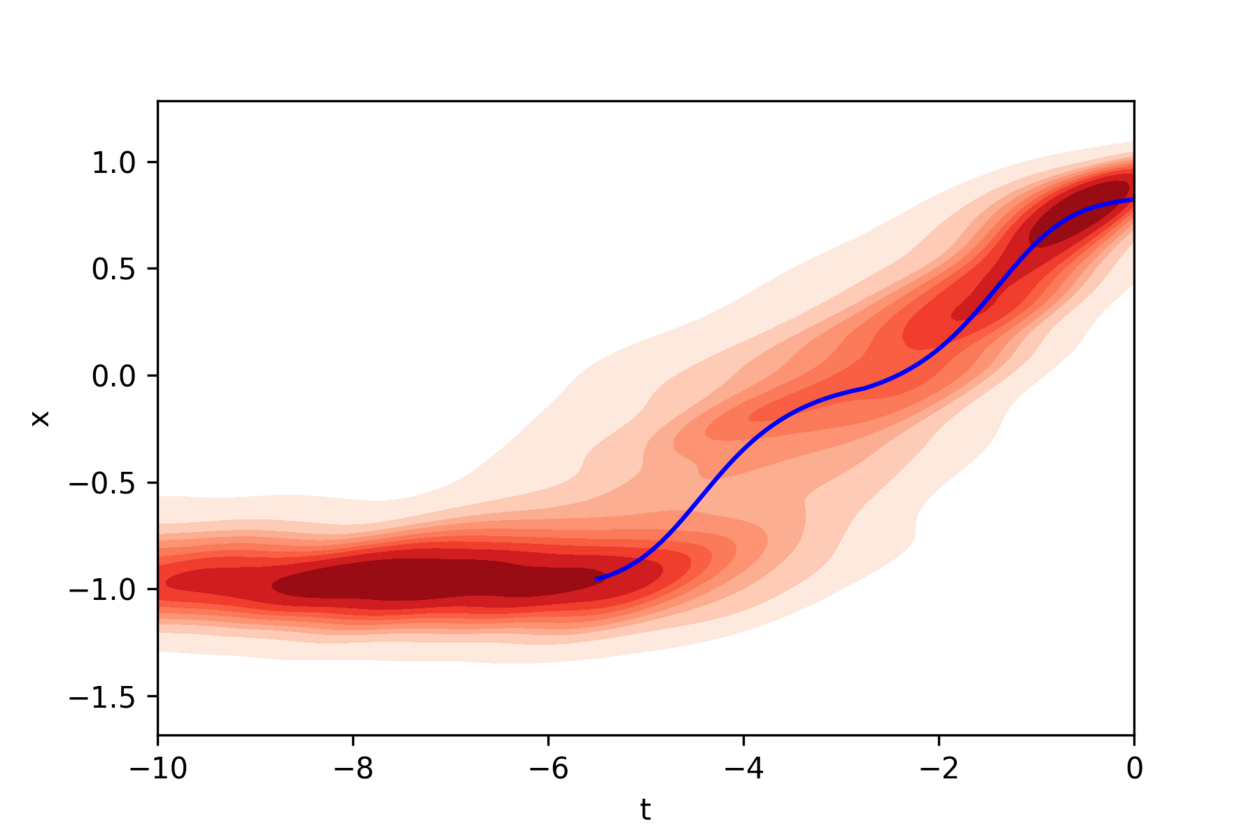
\includegraphics[width=0.5\textwidth]{figures/lez_12_walker_t_theory.png}
    \caption{\scriptsize Confronto tra simulazione dei camminatori e curva teorica di un camminatore che minimizza l'azione (\href{https://github.com/dodogabrie/Sistemi-Complessi/blob/master/python-project/lezione12/MFPT_simulation_py.ipynb}{Link al codice in python}).}
    \label{fig:figures-lez_12_walker_t_theory-png}
\end{figure}
\noindent
Notiamo che la curva teorica è compatibile con il flusso di camminatori
\footnote{Sul plot è necessario precisare che il camminatore con la legge $\dot{x} = \pm U'$ raggiunge i punti interessanti $x=0$, $x=+1$ in un tempo infinito. Il moto è stato tagliato per renderlo ragionevolmente simile all'andamento delle simulazioni. Guardando il file del professore suppongo abbia fatto lo stesso. Questo falsifica parzialmente la validità del risultato.
}
.\\
Risolvendo le equazioni di Hamilton per $p (=\lambda)$ si ottiene anche il seguente andamento teorico:
\begin{figure}[H]
    \centering
    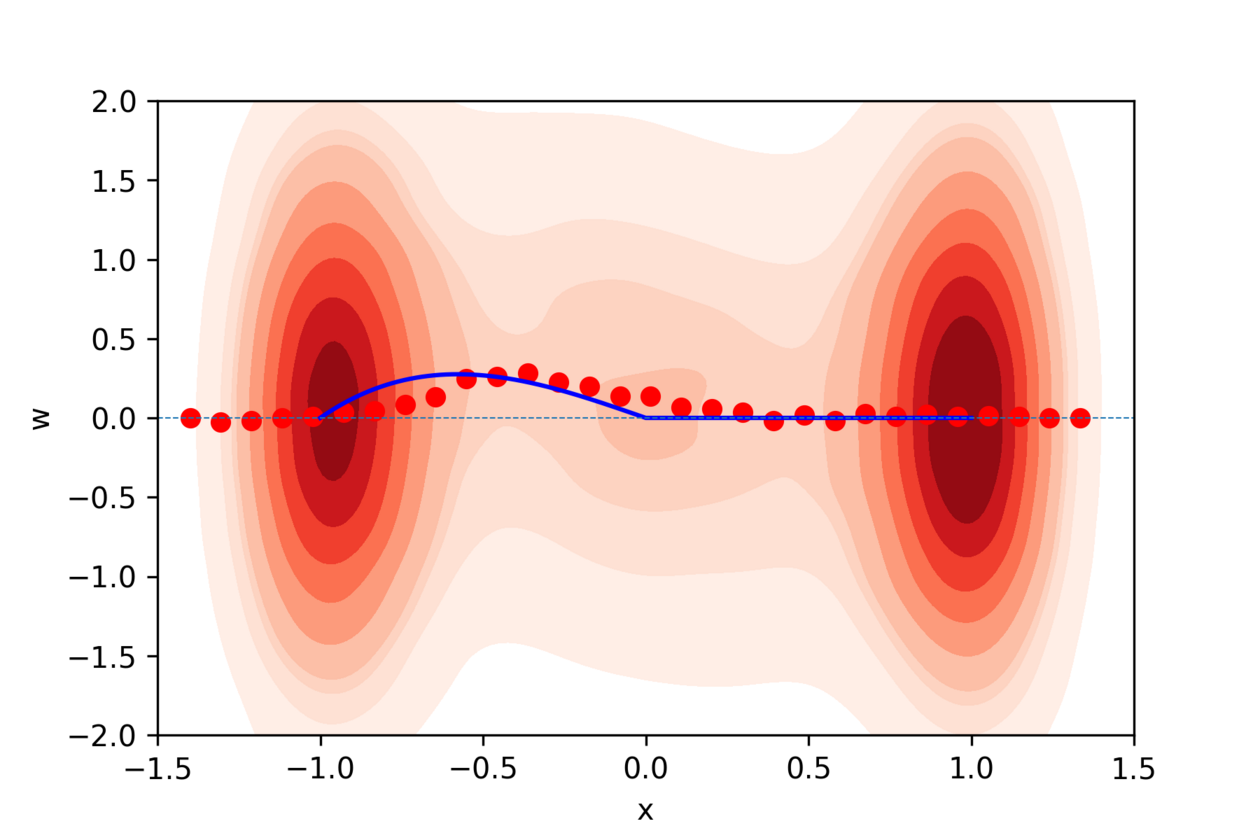
\includegraphics[width=0.5\textwidth]{figures/lez_12_dist_theory.png}
    \caption{\scriptsize Confronto tra media predetta del processo di Wiener e media ottenuta dalle simulazioni, tutto in funzione di $x$ (\href{https://github.com/dodogabrie/Sistemi-Complessi/blob/master/python-project/lezione12/MFPT_simulation_py.ipynb}{Link al codice in python}).}
    \label{fig:figures-lez_12_dist_theory-png}
\end{figure}
\noindent
Per ottenere questo risultato è stato necessario, a livello computazionale, di moltiplicare la soluzione $p$ per il fattore $dt / \sqrt{\epsilon}$. 
Senza far questo il rumore ottenuto verrà fuori scala rispetto a quello simulato.\\
Possiamo notare una non conformità nei pressi di $x=0$, questo può essere dovuto al campione statistico di simulazioni
\footnote{Noto che il campione può essere ampliato scrivendo una funzione e chiamandola più volte. In questo modo si risolve il problema della memoria occupata in eccesso a causa della matrice di numeri random e di quella delle posizioni iniziali.}.\\
Possiamo adesso utilizzare questo modello per confrontarlo con le simulazioni. In figura \ldots si mostra una simulazione di camminatori che raggiungono $x= 0.2$ per poi rilassare.
\begin{figure}[H]
    \centering
    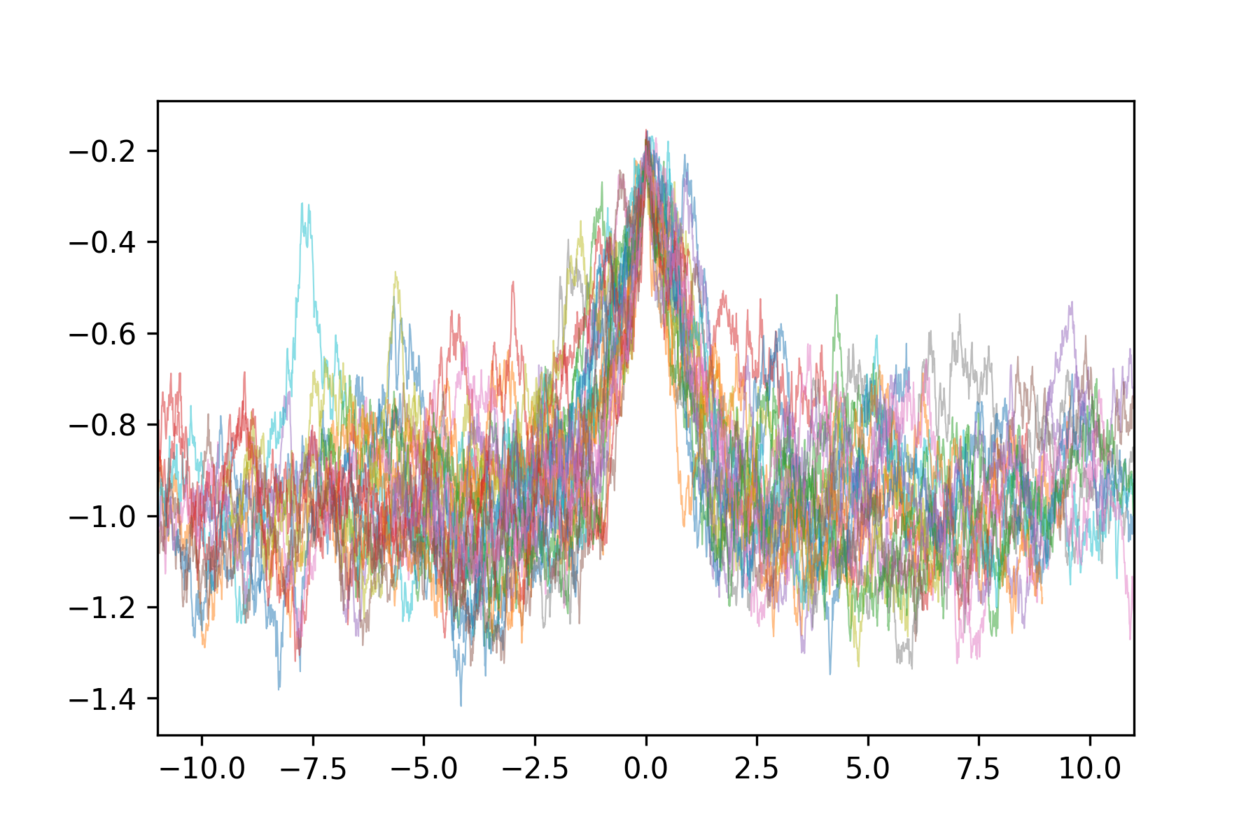
\includegraphics[width=0.5\textwidth]{figures/lez_12_walker_t_cutted.png}
    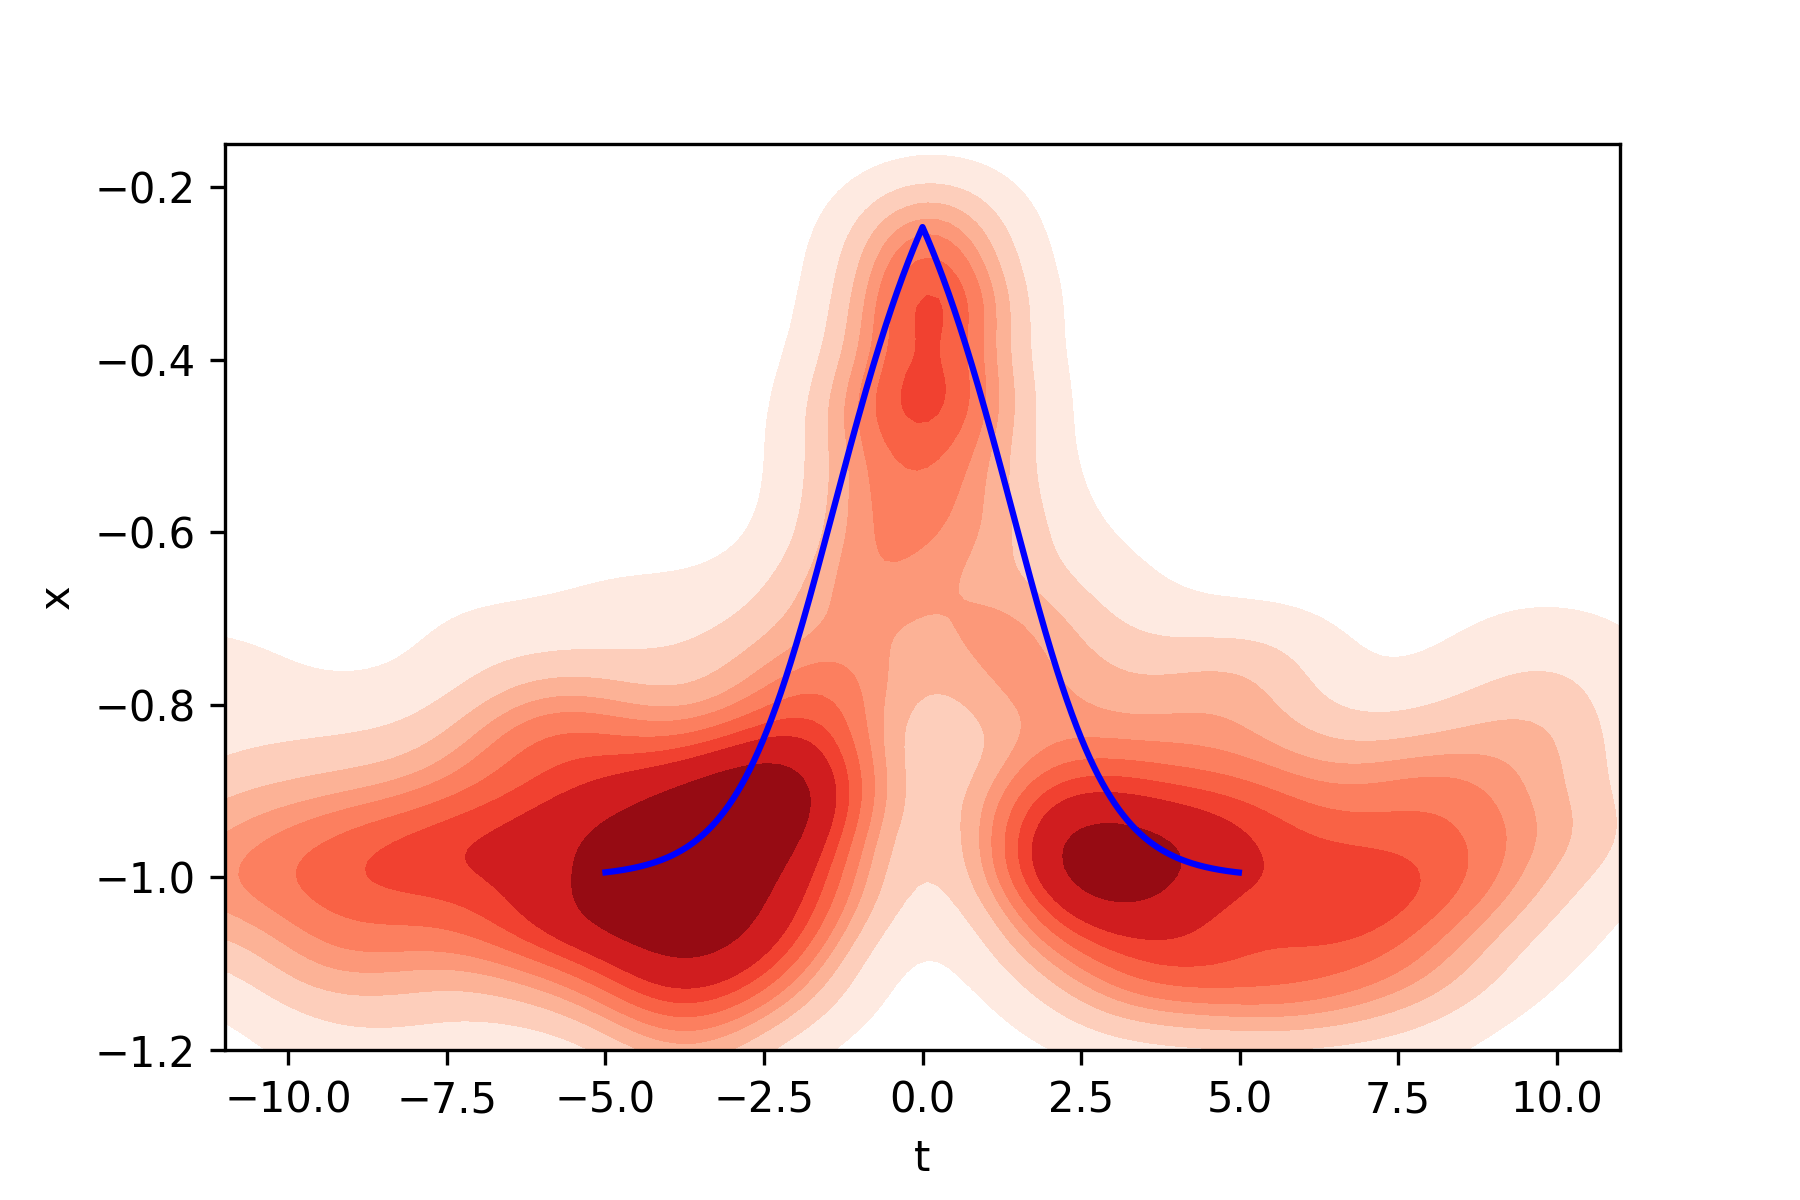
\includegraphics[width=0.5\textwidth]{figures/lez_12_walker_t_cutted_theory.png}
    \caption{\scriptsize Camminatori selezionati che arrivano a $x = 0.2$ per poi rilassare e distribuzione in densità dei camminatori con la curva teorica in blu (\href{https://github.com/dodogabrie/Sistemi-Complessi/blob/master/python-project/lezione12/MFPT_simulation_py.ipynb}{Link al codice in python}).}
    \label{fig:figures-lez_12_walker_t_cutted_theory-png}
\end{figure}
\noindent
Si nota come i camminatori si distribuiscono lungo due cammini che corrispondono a $\dot{x} = \pm U'$.
\subsection{Da cammino ottimale a MFPT}%
\label{sub:Da cammino ottimale a MFPT}
Abbiamo detto che il contributo stocastico arriva solo nella parte di salita, possiamo usare questo per calcolare la derivata della azione:
\begin{equation}
\begin{aligned}
    \dot{S} =& \frac{\partial H}{\partial p} p - H = \\
            =& \left(p-U'\right)p - \frac{1}{2}p^2+pU' = \\
	    =& \frac{1}{2}p^2 = \\
	    =& \frac{1}{2}\left(\dot{x}+U'\right)^2
.\end{aligned}
\label{eq:12_action}
\end{equation}
Sostituendo la soluzione per $\dot{x}$ ottenuta prima si ha che:
\[
    \dot{S} = 
    \begin{cases}
	2(U') ^2 & \text{ Salita}\\
	0        & \text{ Discesa}
    \end{cases}
    = 2 \dot{x}^2 = 2\dot{x}U'
.\] 
A questo punto possiamo integrare per ottenere l'azione:
\[\begin{aligned}
    S_{min} =& \int\dot{S}dt = 
             2\cdot \int_{a}^{b} \dot{x}U'dt = \\
            =& 2  \int_{a}^{b} \left(\frac{\text{d} U}{\text{d} t} \right)dt =
	     2(U_b-U_a)  
.\end{aligned}\]
Quindi il tempo di primo passaggio, come già accennato, sarà proporzionale a:
\[\begin{aligned}
    \text{MFPT} \sim& \exp\left(-\frac{S_{\text{min}}}{\epsilon}\right) =
    \exp\left(-\frac{2(U_b-U_a)}{2D}\right) =\\
    =&\exp\left(-\frac{U_b-U_a}{D}\right)
.\end{aligned}\]
Che è proprio la legge di Harrenius trovata nella lezione precedente.\\
Il metodo esposto per il tempo di primo passaggio è molto generale, possiamo applicarlo anche a casi N-dimensionali.
\subsection{Calcolo del MFPT in 2D: Oscillatore di Van Der Pol invertito}%
\label{sub:Calcolo del MFPT in 2D}
Prendiamo un sistema bidimensionale con le seguenti SDE per il moto dei camminatori:
\[\begin{aligned}
    & dx = ydt\\
    & dy = \left(-2\eta (1-x^2) y - x\right)dt + \sqrt{ 4\eta T} d\omega
.\end{aligned}\]
Questo sistema è un famoso oscillatore, studiato per descrivere l'andamento della corrente nelle valvole.
\begin{figure}[H]
    \centering
    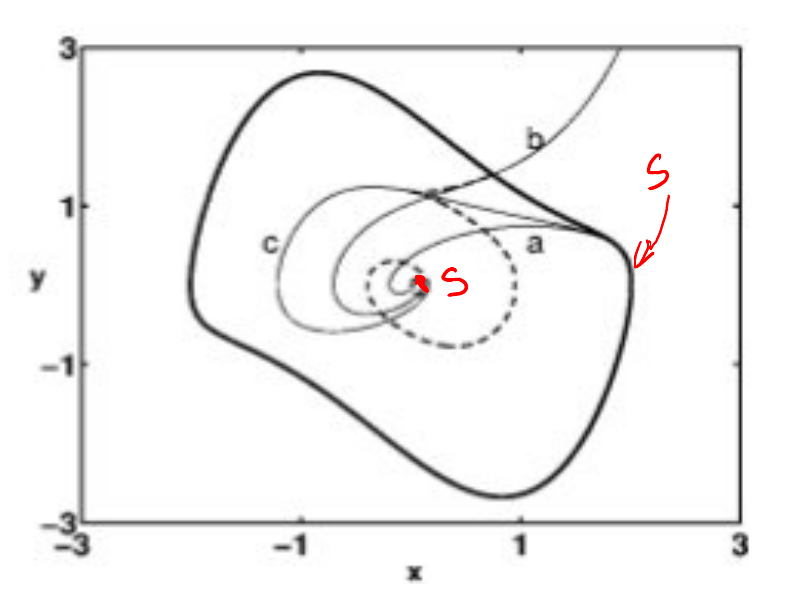
\includegraphics[width=0.4\textwidth]{figures/lez_12_Van_Der_Pol_oscillator.png}
    \caption{\scriptsize Oscillatore di Van Der Pole nello spazio $x, y$.}
    \label{fig:figures-lez_12_Van_Der_Pol_oscillator-png}
\end{figure}
\noindent
La linea scura in figura è un \texttt{Ciclo limite instabile}, inserendo un camminatore in questa traiettoria ( con le condizioni iniziali opportune e rimuovendo la parte stocastica della equazione ) questo rimarrebbe eternamente su di essa. Un camminatore che parte all'interno collassa sull'origine $S$, all'esterno invece i punti scappano via verso $r\to \infty$.\\
Possiamo immaginare quindi questo sistema come un potenziale dalla forma "vulcanica", in cui il ciclo limite instabile corrisponde al cratere.\\
Possiamo chiederci quanto impieghi un camminatore inizializzato all'interno ad arrivare sul bordo del cratere ( come risalire un potenziale bidimensionale ).\\
Potremmo tentare di risolvere il problema come fatto in precedenza:
\begin{itemize}
    \item Trovare l'equazione di FK.
    \item Scrivere l'equazione del tempo di primo passaggio.
    \item Risolvere l'equazione alle derivate parziali.
\end{itemize}
Il problema è che, anche se si riuscisse a risolvere l'equazione alle derivate parziali, non è affatto banale inserire le condizioni al contorno (ne analiticamente ne numericamente).\\
Il vantaggio del metodo è che possiamo scrivere una Hamiltoniana per il sistema:
\[
    H = yp_x + \left[-2\eta (1-x^2) y - x\right]p_y + \frac{1}{2}(4\eta T) p_y^2
.\] 
Possiamo dire che i camminatori partono dal fondo del cratere $S$, si risolve il problema trovando i cammini che arrivano al bordo del cratere e poi si minimizzano questi cammini (si minimizza l'azione). \\
Le traiettorie $a$, $b$ in figura \ref{fig:figures-lez_12_Van_Der_Pol_oscillator-png} sono state trovate dal professore ed arrivano tangenti al ciclo limite.\\
Possiamo cercare di capire se il sistema ha una distribuzione di equilibrio, questo equivale a capire se il sistema presenta il bilancio dettagliato.\\
La condizione del bilancio dettagliato è soddisfatta se vale la \ref{eq:11_rot}. Esplicitando tale conto si ha:
\[
    f_x = y \qquad f_y = -2\eta (1-x^2) y - x
.\] 
\[
    \frac{\partial f_x}{\partial y} = 1 \neq \frac{\partial f_y}{\partial x} = 4\eta xy - 1
.\] 
L'equazione al rotore nullo non è soddisfatta, quindi il sistema non presenta il bilancio dettagliato.\\
L'assenza del bilancio dettagliato non influisce sul calcolo del MFPT, tuttavia la traiettoria di fuga ottimale non è univoca (come invece si avrebbe con il bilancio dettagliato) e di conseguenza si sviluppa una cuspide all'interno del ciclo limite instabile (nello spazio delle fasi vediamo più di un cammino partendo dallo stesso punto).
\begin{exmp}[]
    Prendiamo la seguente SDE:
    \[
	 dx = (-U'(x) + A\sin (wt) ) dt + \sqrt{\epsilon} d\omega    
    .\] 
    La possiamo spezzare in due termini:
    \[
	\begin{cases}
	 dx_1 = w dt\\
	 dx_2 = (-U'(x_2) + A\sin (x_1) ) dt + \sqrt{\epsilon} d\omega    
	\end{cases}
    \] 
    Le equazioni di Hamilton-Jacobi ricordiamo essere:
    \[
        \begin{cases}
            \dot{x}= -U' + p\\
	    \dot{p} = U'' p
        \end{cases}
    \] 
    Essendo in due dimensioni non abbiamo quantità scalari, ad esempio:
    \[
        -U' = 
	\begin{pmatrix} 
	    w  \\
	    A\sin (x_1) -U'(x_2) 
	\end{pmatrix} 
    \] 
    Quindi esisterà anche un tensore delle derivate seconde, le cui componenti non nulle sono:
    \[\begin{aligned}
	& U''_{x_1, 2} = -\partial_{x_1}w + \partial_{x_1}(A\sin (x_1)) = -A\cos (x_1) \\
	& U_{x_2,2} = -\partial_{x_2} (-U'(x_2) ) 
    \end{aligned}\]
    In cui si è cambiato segno perché avevamo $-U'$. Alla fine si ottiene un oggetto del tipo:
    \[
        U'' = 
	\begin{pmatrix} 
	    0  &  -A\cos (x_1) \\
	    0  &  d^2U/d(x_2)^2
	\end{pmatrix} 
    .\] 
    In conclusione abbiamo il seguente set di equazioni per il moto:
    \[\begin{aligned}
	&\dot{x}_1 = w\\
	&\dot{x}_2 = -U'(x_2) + A \sin (x_1) + p_2 \\
	& \dot{p}_1 = -A\cos (x_1) \cdot p_2\\
	& \dot{p}_2 = \frac{\text{d}^2}{\text{d} (x_2)^2 }(U) \cdot  p_2
    .\end{aligned}\]
    L'Hamiltoniana si scrive come:
    \[
	H = w p_1 + \frac{(p_2)^2}{2} + p_2(A\sin (x_1) - U'(x_2) ) 
    .\] 
    Ricordiamo che di ha questa forma perché dev'essere:
    \[
        \frac{\text{d} p}{\text{d} t} = - \frac{\partial H}{\partial q}  
	\qquad \qquad
	\frac{\text{d} q}{\text{d} t} = \frac{\partial H}{\partial p} 
    .\] 
    Possiamo estrarre l'azione dalla \ref{eq:12_action}, si ottiene:
    \[\begin{aligned}
	\dot{S} = p\partial_{p}H-H=\ldots=\frac{(p_2)^2}{2}
    .\end{aligned}\]
    Simulando il moto con le equazioni di Hamilton si possono ottenere delle traiettorie come quelle in Figura \ref{fig:figures-lez_12_strange_motion-png}.
    \begin{figure}[H]
        \centering
	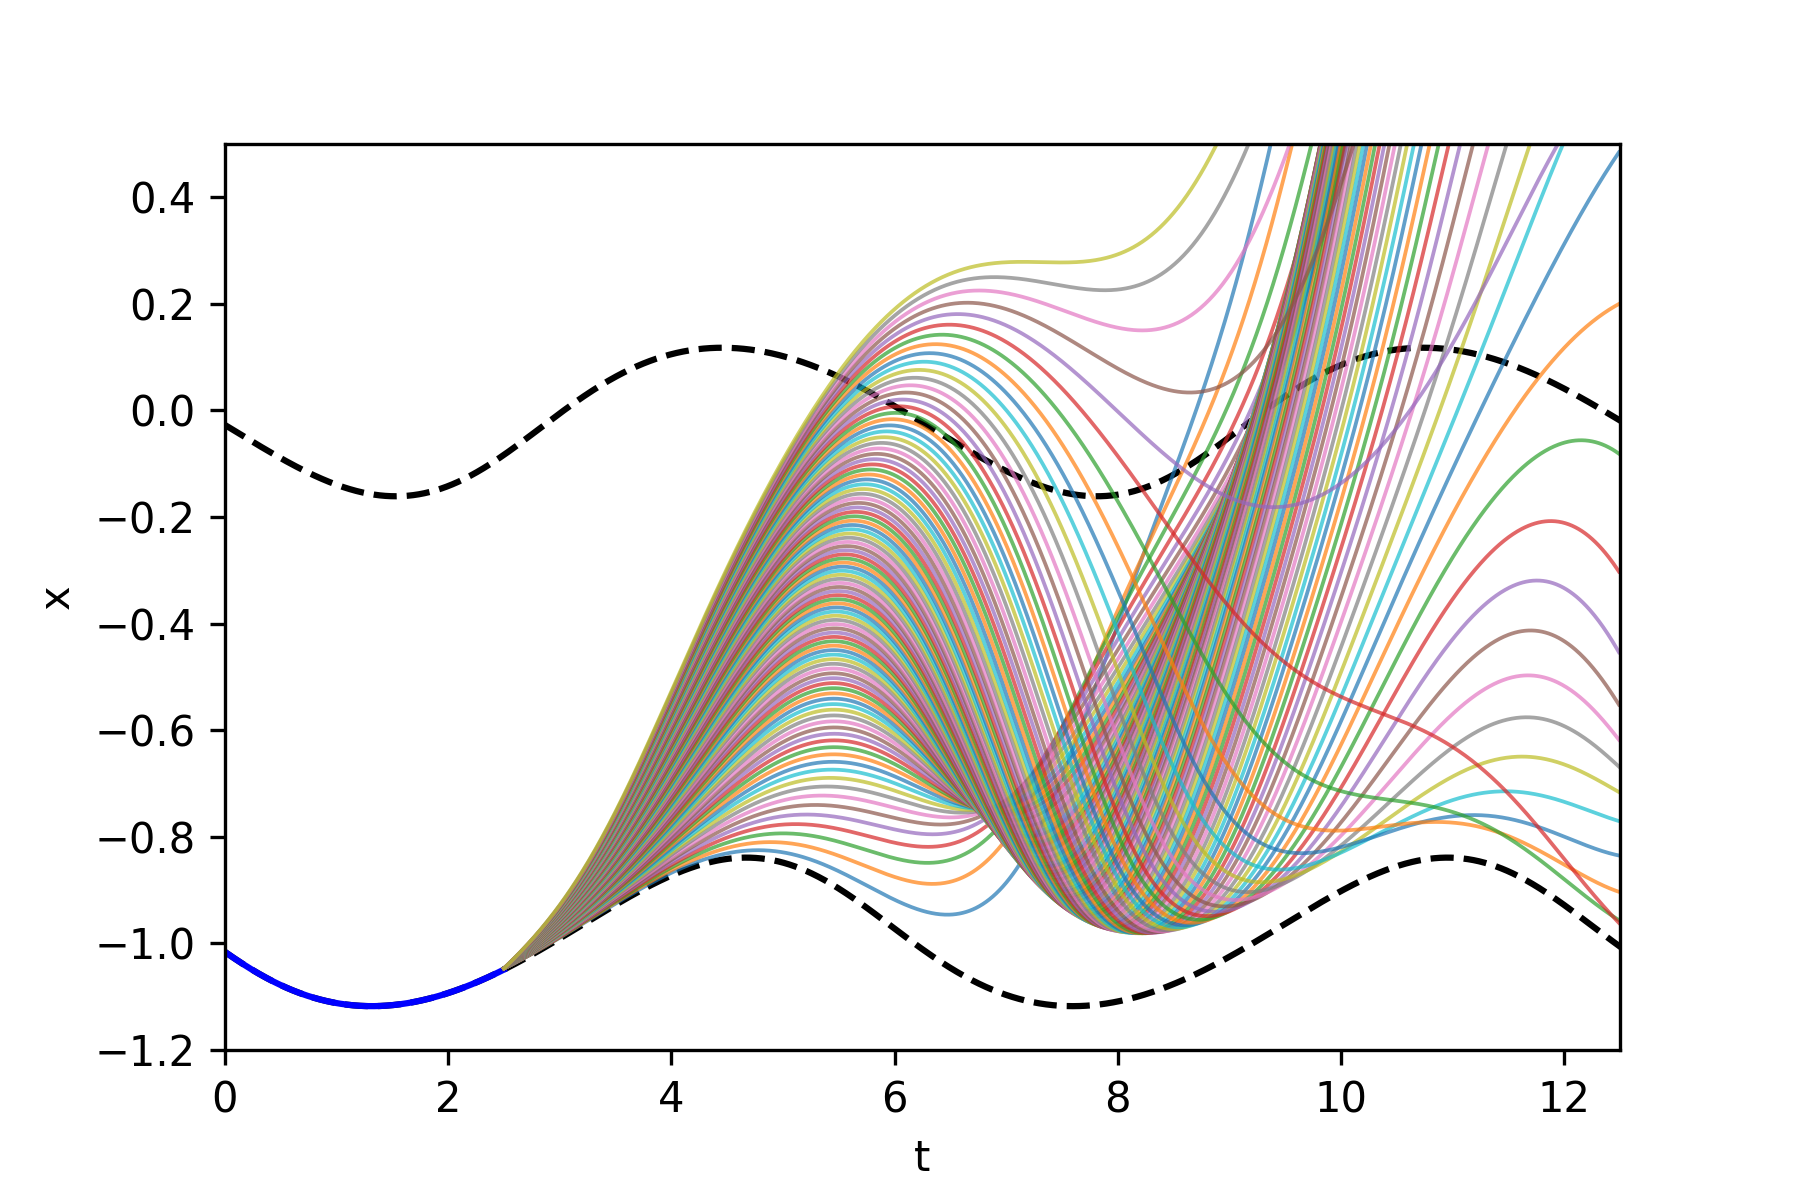
\includegraphics[width=0.5\textwidth]{figures/lez_12_strange_motion.png}
	\caption{\scriptsize Traiettorie di fuga generate con le equazioni del moto. La traiettoria che minimizza l'azione (tra le condizioni iniziali testate) è evidenziata in rosso. Notiamo per arrivare in un punto nei pressi della cuspide ci siano più traiettorie possibili, questo è tipico dei sistemi che non hanno il bilancio dettagliato.}
        \label{fig:figures-lez_12_strange_motion-png}
    \end{figure}
    \noindent
    Per generare tali traiettorie c'è bisogno di un "delicato" lavoro computazionale.
    Creare la routine per i camminatori è semplice, meno semplice è la scelta delle condizioni iniziali.
    Il sistema è estremamente sensibile alla scelta di $w, A$ e tutte le variabili del moto $p_i, x_i$. \\
    Alcune traiettorie in figura sembrano rilassare, questa è solo una "illusione", infatti nelle oscillazioni successive le traiettorie fuggono tutte, d'altronde il modello scelto serve "solo" a descrivere le traiettorie di fuga.\\ 
    Avendo la sequenza dei $p_2$ è possibile calcolare anche l'azione complessiva su ogni percorso, il risultato che si ottiene è il seguente:
    \begin{figure}[H]
        \centering
	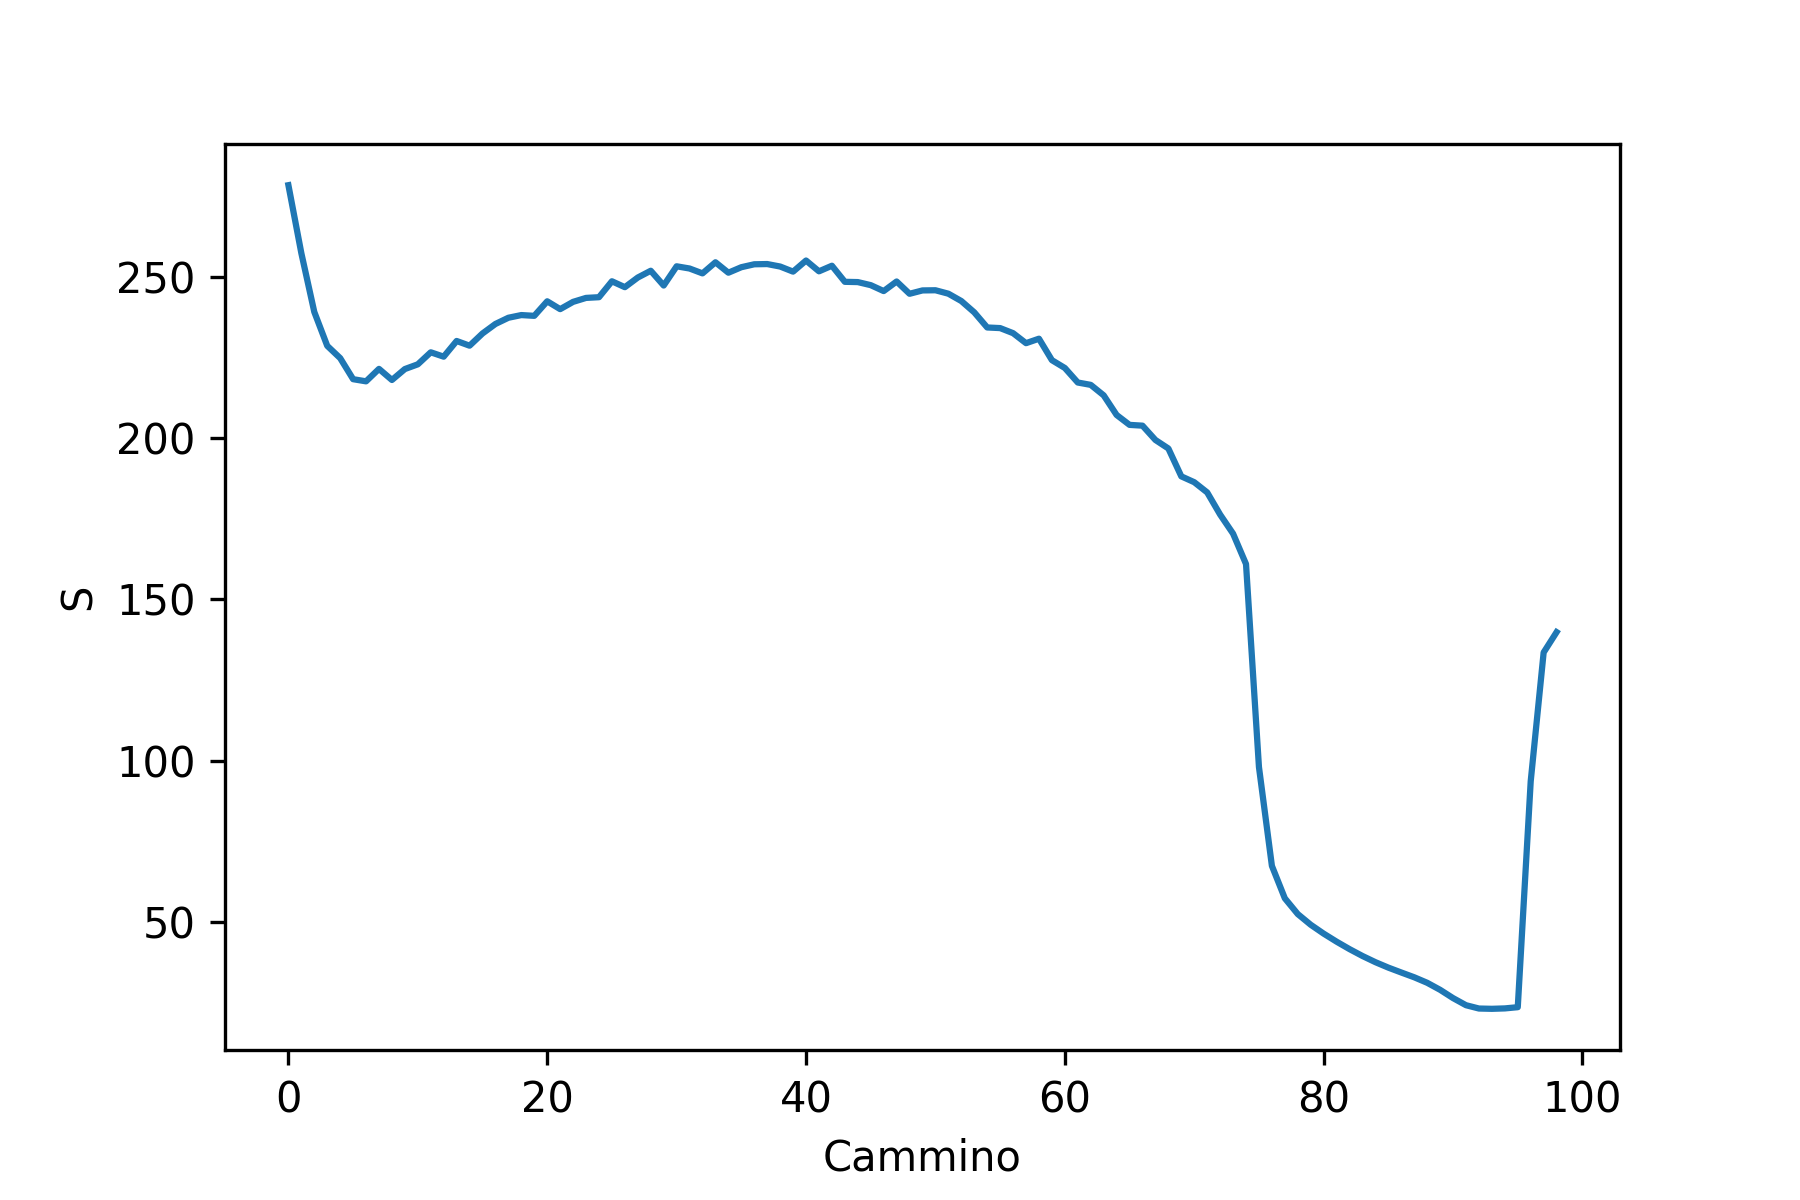
\includegraphics[width=0.5\textwidth]{figures/lez_12_strange_motion_action.png}
	\caption{\scriptsize Azione al variare del camminatore i-esimo. Notiamo l'evidenza di un minimo corrispondente alla curva rossa in figura \ref{fig:figures-lez_12_strange_motion-png}. La possibilità di stimare l'azione minima permette il calcolo del tempo di primo passaggio.}
        \label{fig:figures-lez_12_strange_motion_action-png}
    \end{figure}
    \noindent 
    Il grafico precedente non rispecchia a pieno la vera azione di tutti i camminatori in quanto tutti i moti che scappano dal sistema sono stati troncati per evitare l'overflow, tuttavia possiamo affermare che l'azione di questi camminatori fuggenti è stata sicuramente sottostimata osservando le equazioni di Hamilton.
\end{exmp}
\noindent
Il metodo per trovare le traiettorie di fuga (e quindi il MFPT) è molto potente quando il sistema presenta un "contorno" complicato, può essere applicato addirittura ad un bordo frattale come il set di Julia.
\begin{ex}[Camminatore con bordo dato dal set di Julia]
    Il set di Julia è un bordo frattale, le equazioni agli incrementi per il set sono:
    \[\begin{aligned}
	&x_{n+1} = x^2_n - y^2_n + ax_n + \xi_{x_n}\\
	& y_{n+1}= 2x_ny_n + ax_n + by_n + \xi_{y_n}
    .\end{aligned}\]
    In cui si inserisce un rumore per entrambi gli assi tale che:
    \[
        \left<\xi_{i_n}\xi_{j_n}\right> = \epsilon\delta_{ij}\delta_{nm}
    .\] 
    Il metodo si applica anche a questo bordo senza problemi, se si prova a fare il calcolo si ottiene:
    \begin{figure}[H]
        \centering
	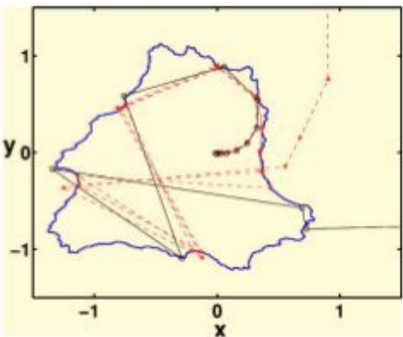
\includegraphics[width=0.4\textwidth]{figures/lez_12_Julia_set.png}
	\caption{\scriptsize Set di Julia con cammino di fuga teorico (tratteggiato) e simulato (nero sottile).}
        \label{fig:figures-lez_12_Julia_set-png}
    \end{figure}
    \noindent
\end{ex}
\noindent
\begin{exmp}[Processo di Ornstein-Ulhenback]
   Se prendiamo un processo di OU possiamo fare gli stessi ragionamenti dell'esempio precedente, partiamo dalle equazioni del processo:
   \[\begin{aligned}
       & dx = f(x) dt + y dt \\
       & dy = - \gamma  y dt + \gamma\epsilon dW
   .\end{aligned}\]
   Risolvendo si arriva alle equazioni di Hamilton-Jacoby:
   \[\begin{aligned}
       & \dot{x}=f(x) + y\\
       & \dot{y}= -\gamma y + p_y\\
       & \dot{p}_x = -f'(x) p_x\\
       & \dot{p}_y=p_x - \gamma p_y
   .\end{aligned}\]
   Ed il problema è risolto.
\end{exmp}
\noindent
\subsection{MFPT applicato allo studio delle glaciazioni}%
\label{sub:MFPT applicato allo studio delle glaciazioni}
Si è notato che l'alternanza tra glaciazioni e periodi caldi ha lo stesso periodo della variazione dell'eccentricità dell'orbita terrestre.\\
Possiamo fare una premessa: la temperatura della terra subisce un feedback negativo per le variazioni di temperatura.
\begin{itemize}
    \item Se la temperatura diminuisce cade la neve ed aumenta il potere riflettente della terra, quindi la temperatura diminuisce ancor di più.
    \item Se la temperatura aumenta il ghiaccio si scioglie e si ha il viceversa.
\end{itemize}
Quindi possiamo immaginare la funzione che determina la temperatura sulla terra come un potenziale a doppia buca (sempre lui, Figura \ref{fig:double_hole_pot}) i quali minimi corrispondono al periodo di caldo e di freddo.\\
Quello che potrebbe fare l'eccentricità è abbassare o alzare uno dei due minimi in funzione della distanza dal sole.\\
Possiamo allora scrivere delle equazioni per la probabilità di essere nel caldo o nel freddo come:
\[\begin{aligned}
    &\dot{P}_f = - \omega_{fc}P_f + \omega_{cf}P_c\\
    & \dot{P}_c =  +\omega_{fc}P_f - \omega_{cf}P_c
.\end{aligned}\]
In cui le $\omega_{ij}$ sono le probabilità di passare da $i$ a $j$.
Visto che l'eccentricità è oscillante possiamo modellizzare questa probabilità con una oscillazione avente lo stesso periodo della eccentricità:
\[
    \omega_{fc /cf} \sim \exp\left(-\frac{U}{T}\mp \frac{A\cos (wt) }{T}\right)
.\] 
Con $T$ temperatura media.\\
Adesso sfruttiamo la proprietà:
\[
    P_f + P_c = 1
.\] 
E approssimiamo l'esponenziale di $\omega$ per temperature grandi ($\gamma_0 = \exp (-U /T)$)
\[
    \omega_{fc/cf} = \gamma_0\left(1\mp \frac{A\cos wt}{T}\right)
.\] 
E si risolvono le equazioni differenziali (di un oscillatore smorzato con una forzante periodica)\ldots Si arriva alla conclusione che:
\[
    P_f = P_0 + \alpha_1 \cos (wt) + \alpha_2 \sin (wt) 
.\] 
Supponendo che in partenza la probabilità di esser caldo o freddo sia la stessa si ha $P_0 = 1 /2$, la cosa importante sono le costanti $\alpha_i$.\\
Andando a calcolare queste \ldots se ne conclude che:
\[
    \left|P_f\right| \sim \sqrt{\alpha_1^2+\alpha_2^2} = \frac{A\gamma_0}{T}\frac{1}{\sqrt{ w^2 + 4\gamma_0^2} }
.\] 
Questa struttura è interessante perché, andando a vedere il rapporto segnale/rumore ($\sim \left|P_f\right| / T$):
\[
    \frac{S}{\text{noise}} \sim \frac{A\gamma_0}{T^2 }\frac{1}{\sqrt{ w^2 + 4\gamma_0^2} }
.\] 
L'andamento di questa funzione non è monotono ma presenta una temperatura ottimale, per tale temperatura si ha una massima probabilità di fare uno switch caldo/freddo in fase con l'eccentricità dell'orbita terrestre (\texttt{Risonanza stocastica}).
\clearpage
